\documentclass{article}

\usepackage{amsmath}
\usepackage{amssymb}
\usepackage{graphicx}
\usepackage[spanish]{babel}
\usepackage{cancel}
\usepackage{enumerate}
\usepackage{hyperref}
\hypersetup{
    colorlinks,
    citecolor=black,
    filecolor=black,
    linkcolor=black,
    urlcolor=black,
}
\usepackage{tcolorbox}
\usepackage{xcolor}

\tcbuselibrary{theorems}

\newcommand{\hresult}[2]{\tcboxmath[colback=orange!25!white,colframe=orange, title=#1] {#2} }
\newcommand{\hresulte}[3]{\tcboxmath[colback=orange!25!white,colframe=orange, title=#1] { \hspace{#3} #2 \hspace{#3} } }

\renewcommand{\Bbb}{\mathbb}

\title{Ejercicios de Análisis Matemático CBC (28) \\
Práctica 1: Funciones reales \\
Cátedra Ruiz, curso 62802 \\
1° C 2003}
\author{Darío Eduardo Ramos}

\begin{document}
\maketitle

\tableofcontents{}

\newpage

\section*{1}
\label{sec:1}
\addcontentsline{toc}{section}{\nameref{sec:1}}

\textbf{Haga un gráfico que refleje la evolución de la temperatura del agua a lo largo del tiempo atendiendo a la siguiente descripción:}

\vspace{1em}

\textbf{``Saqué del fuego una cacerola con agua hirviendo. Al principio, la temperatura del agua bajó con rapidez, de modo que a los 5 minutos estaba en 60º. Luego fue enfriándose con más lentitud. A los 20 minutos de haberla sacado estaba a 30º y 20 minutos después seguía teniendo algo más de 20º, temperatura de la cual no bajó, pues era la temperatura que había en la cocina.'' }

\vspace{1em}

\textbf{¿Es el gráfico que hizo el único que respeta las consignas anteriores?}

\vspace{1em}

\hrule

\vspace{1em}

Planteando la temperatura como una función del tiempo, llámese $y = f(t)$, los datos que se tienen sobre $f$ son los siguientes:

\begin{subequations}
\begin{align}
& f(t < 0) = 100 \\
& f(0) = 100 \\
& f(5) = 60 \\
& f(20) = 30 \\
& f(40) = 20+ \\
& f(t > 40) = 20
\end{align}
\end{subequations}

Dado que no se tiene una expresión cerrada para $f$, existen infinitas funciones de variable continua que satisfacen estas restricciones. Cualquier gráfico que se haga que pase por los puntos dados y se mantenga constante para $t < 0$ y $t > 40$ con los valores dados es válido. Resulta conveniente definir los grados Celsius como la unidad del eje $y$, y los minutos como la unidad del eje $x$. Por ejemplo:

\newpage

\begin{figure}[ht]
\caption{un gráfico posible}
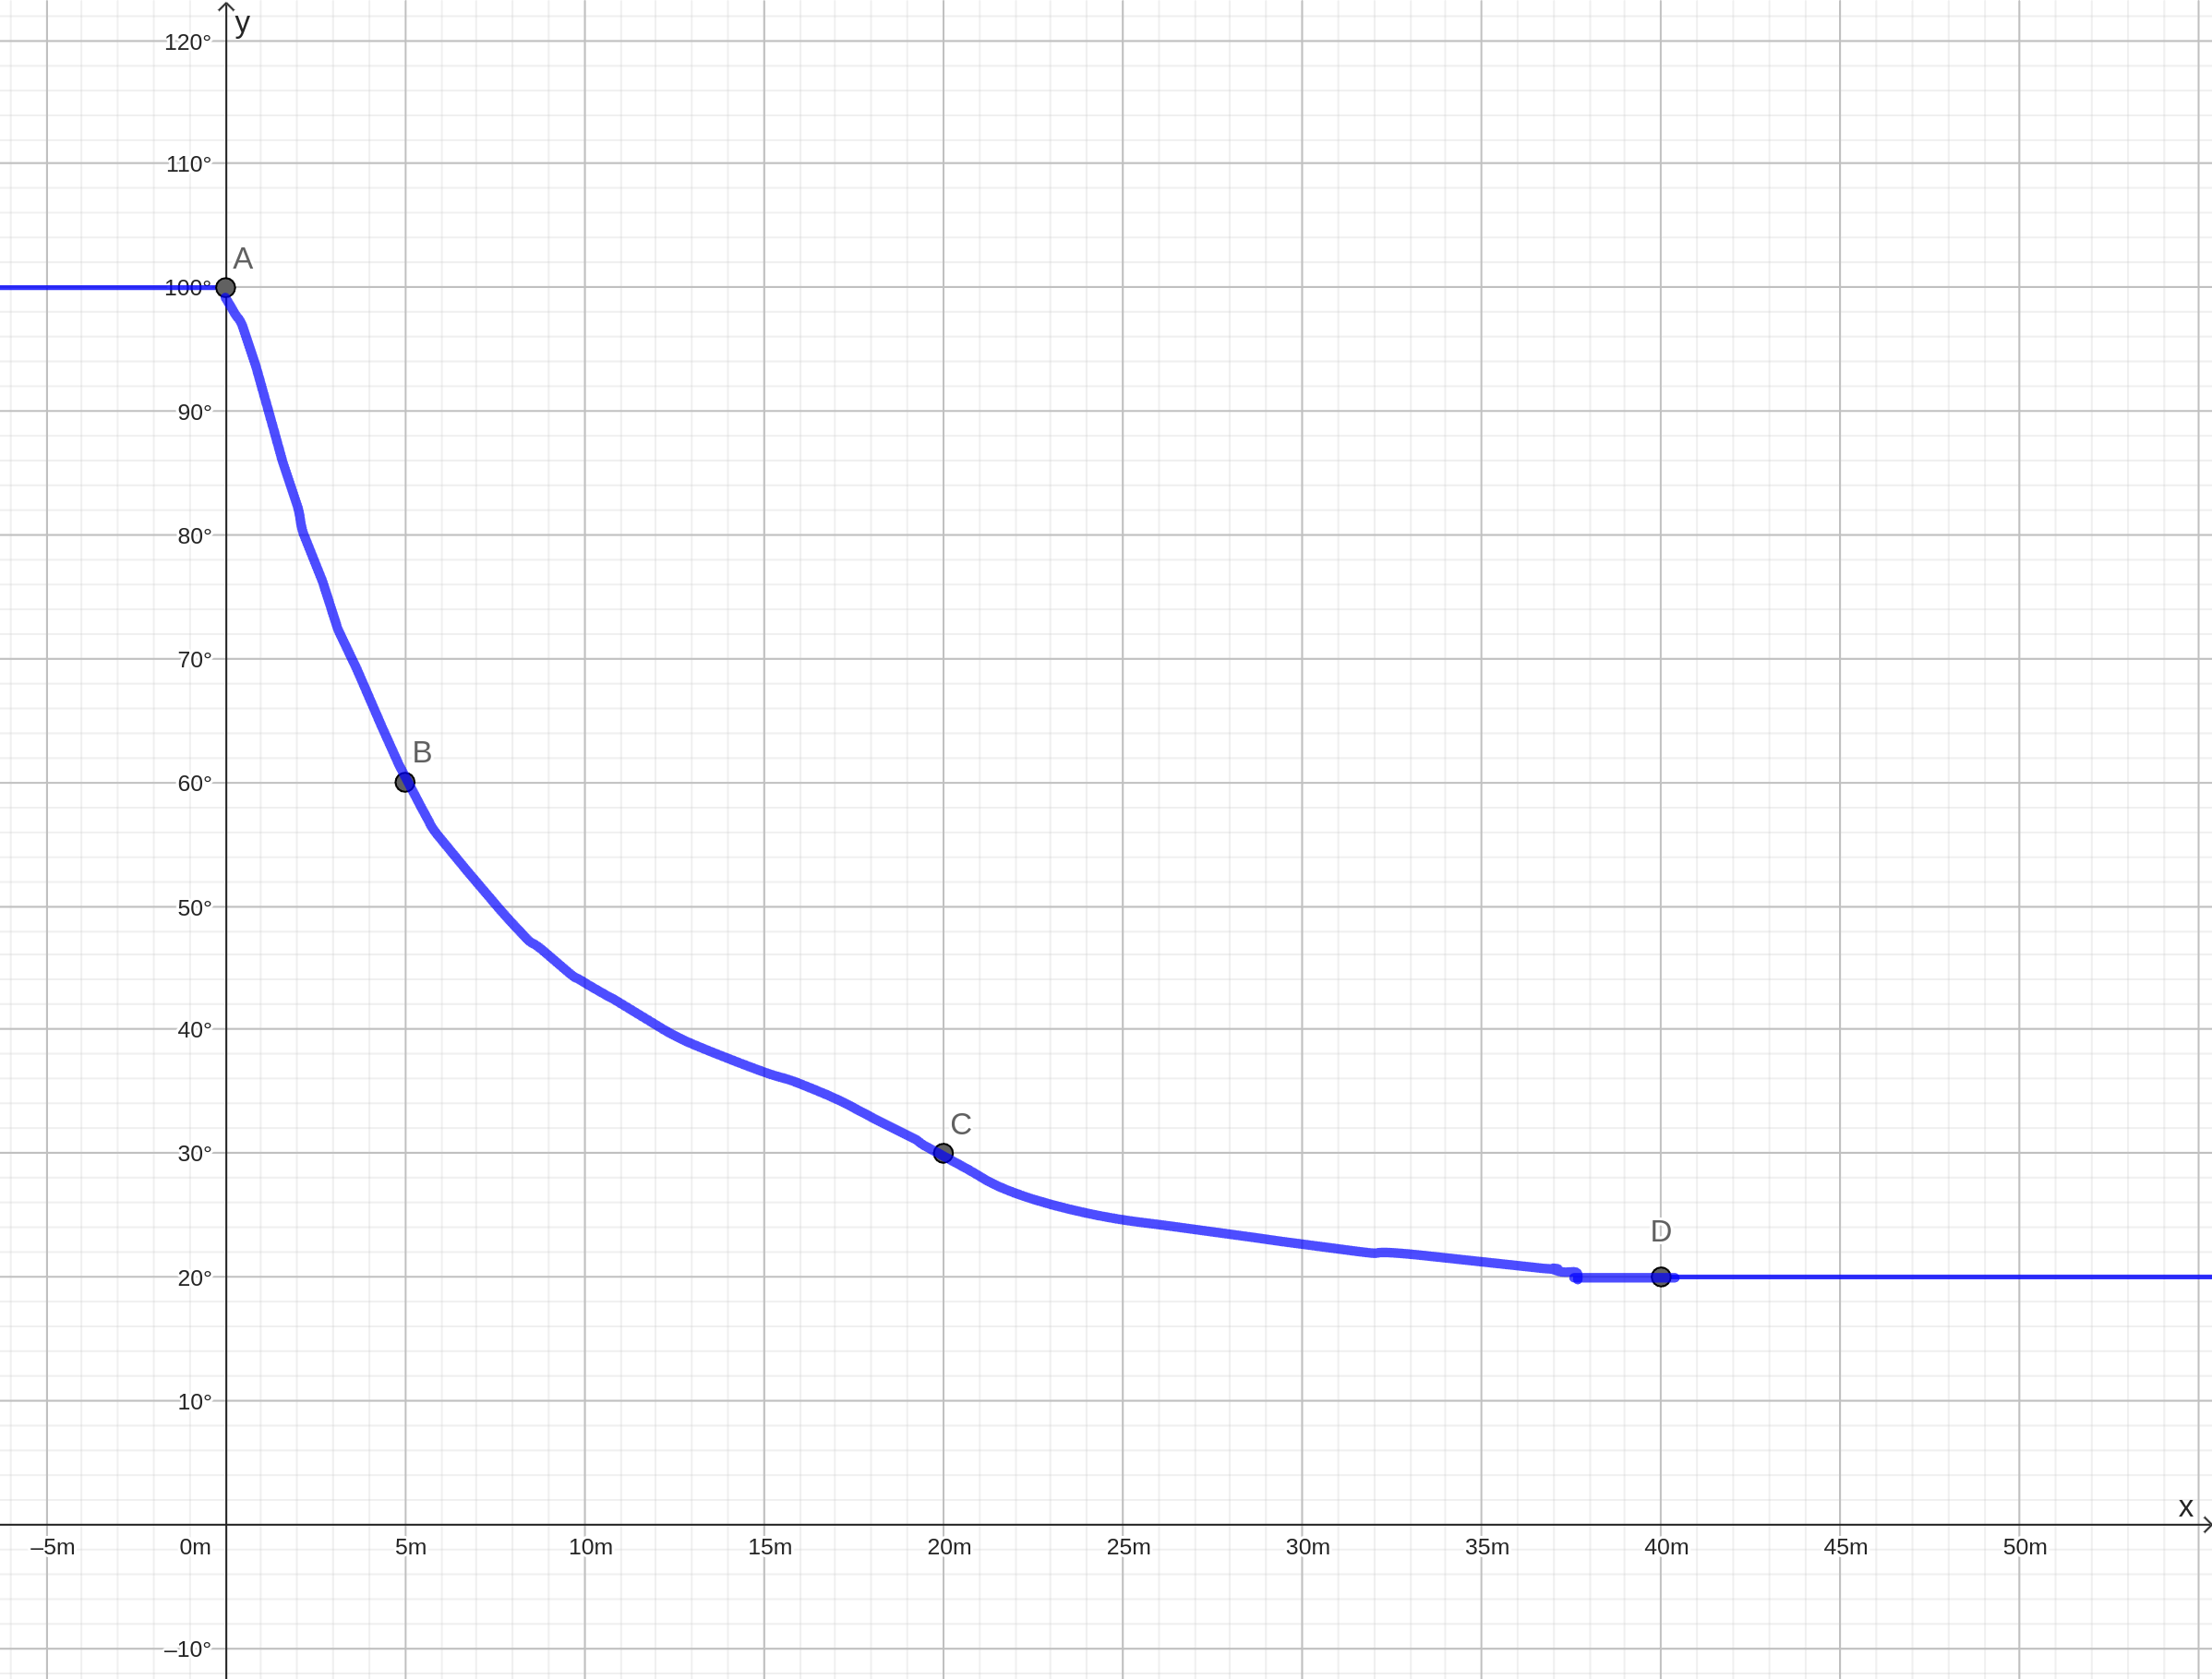
\includegraphics[scale=0.17]{../img/guide_01/ex_01.png} 
\centering
\label{fig:1}
\end{figure}

\section*{2}
\label{sec:2}
\addcontentsline{toc}{section}{\nameref{sec:2}}

\textbf{Con una lámina rectangular de 40 por 30 queremos hacer una caja como muestra la figura~\ref{fig:2}}

\begin{figure}[ht]
\caption{}
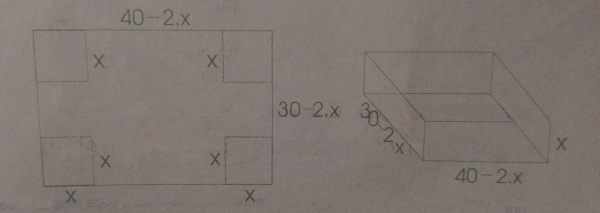
\includegraphics[scale=0.8]{../img/guide_01/ex_02.png} 
\centering
\label{fig:2}
\end{figure}

\begin{enumerate}[(a)]

\item \textbf{Busque la expresión del volumen de la caja en función de $x$. }

\item \textbf{¿Cuál es el dominio?}

\item \textbf{Haga un gráfico aproximado a partir de una tabla de valores.}

\end{enumerate}
\hrule

\subsection*{2.a}
\label{subsec:2.a}
\addcontentsline{toc}{subsection}{\nameref{subsec:2.a}}

El volumen de un cubo no regular, u ortoedro o prisma rectangular, es el área de su base multiplicada por su altura. En este caso:

\begin{equation}
v(x) = (30-2x)(40-2x)x = \hresult{2.a}{ 4x^3 - 140x^2 +1200x }
\end{equation}

\subsection*{2.b}
\label{subsec:2.b}

Exigiendo que todos los lados sean mayores a cero, se obtiene:

\begin{subequations}
\begin{align}
& 30 - 2x > 0 \Rightarrow 30 > 2x \Rightarrow x < 15 \\
& 40 - 2x > 0 \Rightarrow 40 > 2x \Rightarrow x < 20 \\
& x > 0
\end{align}
\end{subequations}

Para que estas tres condiciones se cumplan al mismo tiempo, debe ser:

\begin{equation}
\hresult{2.b}{ \mathop{\text{Dom}}(v) = \{ x \in \mathbb{R} / 0 < x < 15 \} }
\end{equation}

\subsection*{2.c}
\label{subsec:2.c}

La función $v(x)$ es cúbica, con ceros en 0, 15 y 30. Cabe esperar un máximo en el dominio definido, ya que $v(0) = v(15) = 0$.

\begin{center}
\begin{tabular}{||c c||} 
 \hline
 x & v(x) \\ [0.5ex] 
 \hline\hline
 1 & 1064 \\ 
 \hline
 3 & 2448 \\
 \hline
 5 & 3000 \\
 \hline
 7 & 2912 \\
 \hline
 9 & 2376 \\
 \hline
 11 & 1584 \\
 \hline
 13 & 728 \\ [1ex] 
 \hline
\end{tabular}
\end{center}

\newpage

\begin{figure}[ht]
\caption{}
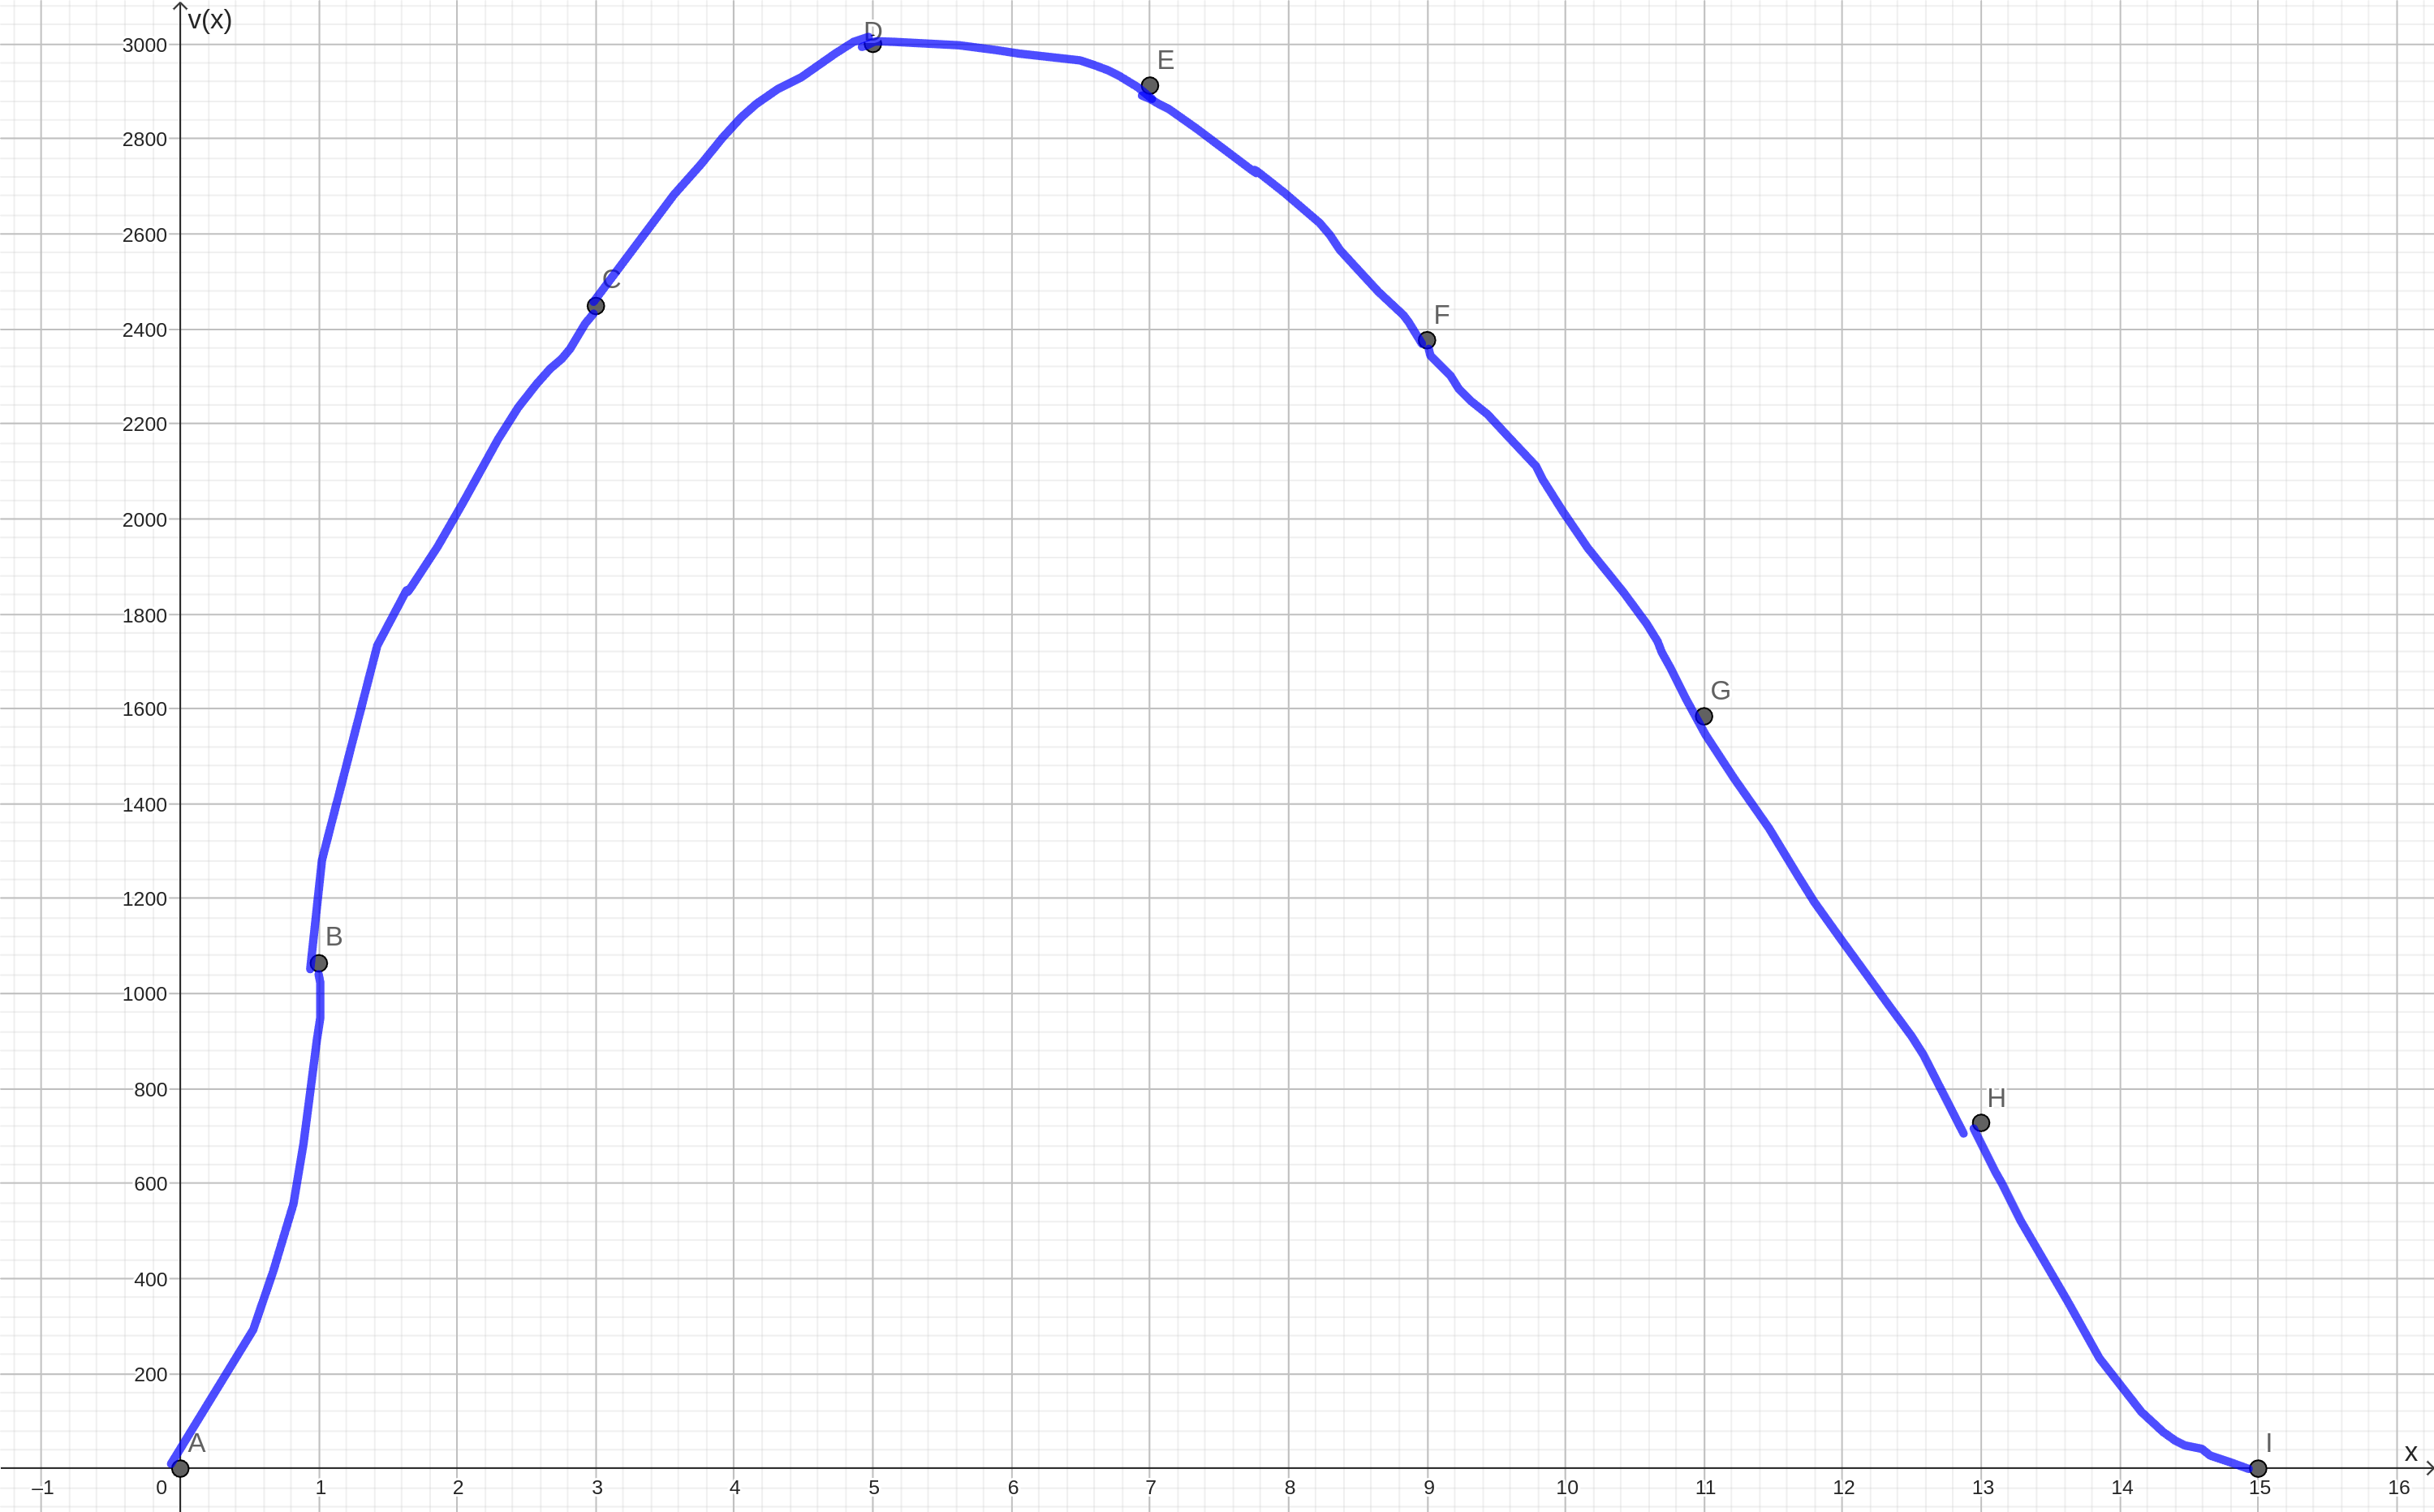
\includegraphics[scale=0.6]{../img/guide_01/ex_02c.png} 
\centering
\label{fig:2c}
\end{figure}

\end{document}
